%# -*- coding:utf-8 -*-
\subsection[冠状动脉分割I]{基于CURVES的冠状动脉分割}

\begin{frame}
\begin{itemize}
\item \textbf{血管介入仿真中冠状动脉表面模型的作用}
\begin{itemize}
\item 虚拟解剖环境的核心组成部分
\item 血管介入术中病灶所在
\item 虚拟导管交互的硬约束
\end{itemize}
\pause \item \textbf{血管介入仿真中冠状动脉表面模型的获取}
\begin{itemize}
\item 几何形状近似的细管
\item 扫描高精度物理模具
\item 医学影像处理方法
\end{itemize}
\pause \item \textbf{冠状动脉的分割与可视化}
\begin{itemize}
\item 是医学影像领域中的一项极具挑战性的工作
\item 形态特征:不规则的空间管状物,走向和半径变化复杂
\item 分割时的主要困难:亮度过低不易观察,细节丢失严重
% \begin{itemize}
% \item 只分割心脏的近似区域,得到近似模型,满足仿真需要
% \end{itemize}
\end{itemize}
\end{itemize}
\end{frame}

\begin{frame}
\begin{itemize}
  \item \textbf{基于CURVES的冠状动脉分割流程}:
\end{itemize}
\begin{figure}[t]
\centering
%# -*- coding:utf-8 -*-
\begin{tikzpicture}[scale=.37]

\draw [black,thick,rounded corners] (-3,0) rectangle (3,2);            % binary threshold
\draw [black,thick,rounded corners] (-3,3) rectangle (3,5);  % CURVES

\draw [black,thick,rounded corners] (-8,7) rectangle (-2,9);   % initial contours

\draw [black,thick,rounded corners] (2,7) rectangle (8,9);     % feature images

\draw [black,thick,rounded corners] (-3,11) rectangle (3,13);  % thresholding
\draw [black,thick,rounded corners] (-3,14) rectangle (3,16);  % curvature anisotropic diffusion
\draw [black,thick,rounded corners] (-3,17) rectangle (3,19);  % raw input

\node [above right] at (-2.25,0.25) {\scriptsize \fs \bf 二值阈值滤波};
\node [above right] at (-2.25,3.25) {\scriptsize \fs \bf 测地活动轮廓};

\node [above right] at (-7.65,7.35) {\scriptsize \fs \bf 初始水平集演进};

\node [above right] at (2.82,7.35) {\scriptsize \fs \bf 特征图像计算};

\node [above right] at (-2.3,11.35) {\scriptsize \fs \bf 二值阈值滤波};
\node [above right] at (-2.9,14.35) {\scriptsize \fs \bf 曲率各向异性扩散};
\node [above right] at (-1.95,17.35) {\scriptsize \fs \bf ROI体数据};

\draw [<-,thick] (0,2) -- (0,3);

\draw [<-,thick] (0,5) -- (0,6);
\draw [thick] (-5,6) -- (5,6);
\draw [thick] (-5,6) -- (-5,7);
\draw [thick] (5,6) -- (5,7);

\draw [<-,thick] (-5,9) -- (-5,10);
\draw [<-,thick] (5,9) -- (5,10);
\draw [thick] (-5,10) -- (5,10);
\draw [thick] (0,10) -- (0,11);

\draw [<-,thick] (0,13) -- (0,14);
\draw [<-,thick] (0,16) -- (0,17);

\end{tikzpicture} 
% 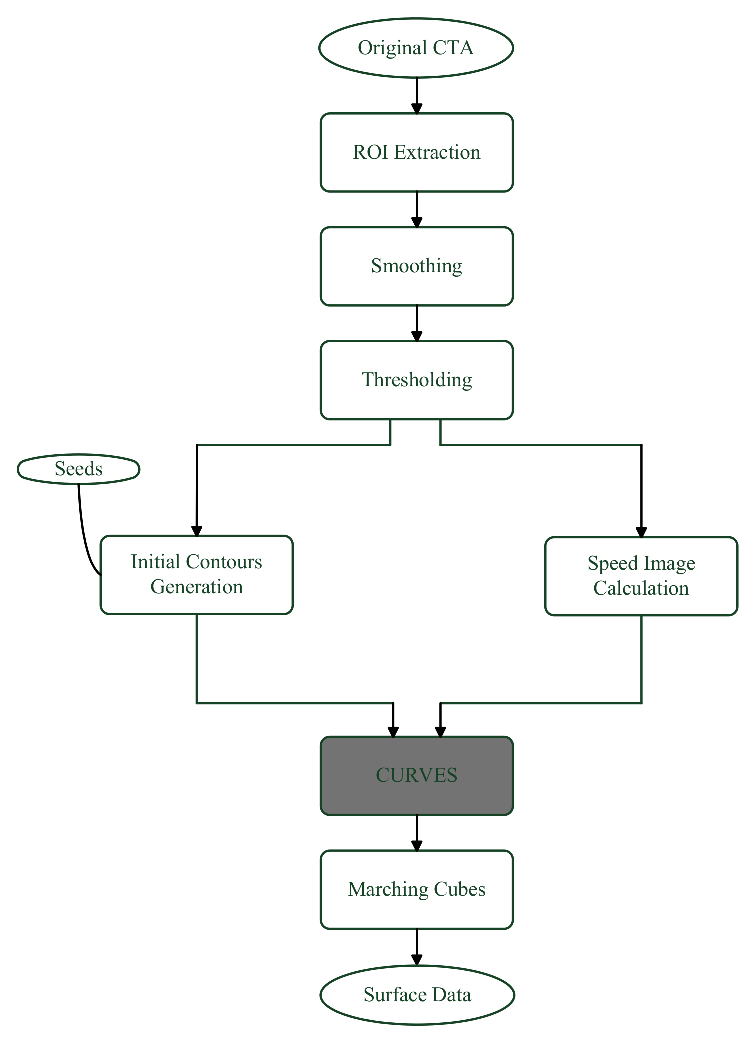
\includegraphics[width=3.2in]{Figures/coronary/DataFlow}
% \caption[心脏区域的ROI提取]{心脏区域的ROI提取。}
% \label{fig:coronary_ROI}
\end{figure}
\end{frame}

\begin{frame}
\begin{itemize}
\item \textbf{CURVES方法~[Lorigo(2001)]}
\begin{itemize}
\item 是GAC的一项扩展,仍属水平集方法
\item 计算准则考虑了目标边缘的平滑性
\item 专门用于探测医学体数据中细微复杂的空间线形结构
% \item 将线形结构的边界抽象为空间流形
\end{itemize}
\pause \item \textbf{CURVES方法的使用}
\begin{itemize}
\item 需要设置计算的起始点
\item 起始点的设置要考虑到冠状动脉的走向
\end{itemize}
\end{itemize}
\end{frame}

\begin{frame}
\begin{itemize}
\item \textbf{CURVES模型}:使如下的能量泛函最小化
\begin{equation*}
% \label{eqn:coronary_CURVES}
E(\mathcal C) = \oint_0^1 g\left( \left| \nabla I \left( \mathcal{C} \left(  s \right) \right) \right| \right) \left| \mathcal{C}'\left( s \right) \right| ds
\end{equation*}
\begin{itemize}
\item $E(\cdot)$:能量泛函
\item $\mathcal{C}(\cdot)$:参数化空间曲线
\item $I(\cdot)$:含有待探测目标的图像
\item $g(\cdot)$:一个严格递减函数,且$g > 0$
\end{itemize}
\end{itemize}
\end{frame}

\begin{frame}
\begin{itemize}
\item \textbf{演进方程}:Euler-Lagrange方程,最速下降法求解
\begin{equation*}
\frac{\partial \mathcal{C}}{\partial t} = k \mathcal{N} - \frac{g'}{g} \varPi \left( \mathcal{H} \frac{\nabla I}{\left| \nabla I \right|} \right)
\end{equation*}
\begin{itemize}
\item $\varPi(\cdot)$:$\mathcal{C}$在其法平面上的投影
\item $\mathcal{H}(\cdot)$:像素亮度函数的Hessian阵
\item $\frac{g'}{g} \left( \mathcal{H} \frac{\nabla I}{\left| \nabla I \right|} \right)$:辅助向量场
\end{itemize}
\end{itemize}
\end{frame}

\begin{frame}
\begin{itemize}
\item \textbf{更新方程}:嵌入水平集空间
\begin{equation*}
\frac{\partial v}{\partial t} = \lambda \left( \nabla v, \nabla^2 v \right) + \frac{g'}{g} \nabla v \cdot \mathcal{H} \frac{\nabla I}{ \left| \nabla I \right| }
\end{equation*}
\begin{itemize}
\item $v(\cdot): \mathrm{R}^3 \rightarrow [0, \infty)$:辅助函数,$\mathcal{C}$的零水平集
\item $\lambda \left( \nabla v, \nabla^2 v \right)$:$P_{\nabla v} \nabla^{2} v P_{\nabla v}$较小的特征值
\item $P_{\nabla v} = I - \frac{\nabla v \nabla v^{T}}{\left| \nabla v \right|^{2}}$:在$\nabla v$法平面上的投影, $I$是像素亮度阵
\end{itemize}
\end{itemize}
\end{frame}

\begin{frame}
\begin{itemize}
  \item \textbf{心脏区域的ROI提取}:
  \begin{itemize}
  \pause \item 设定矩形区域的起点和尺寸
  \pause \item 缩小处理区域,减轻运算负担
  \end{itemize}
\end{itemize}
\begin{figure}[t]
\centering
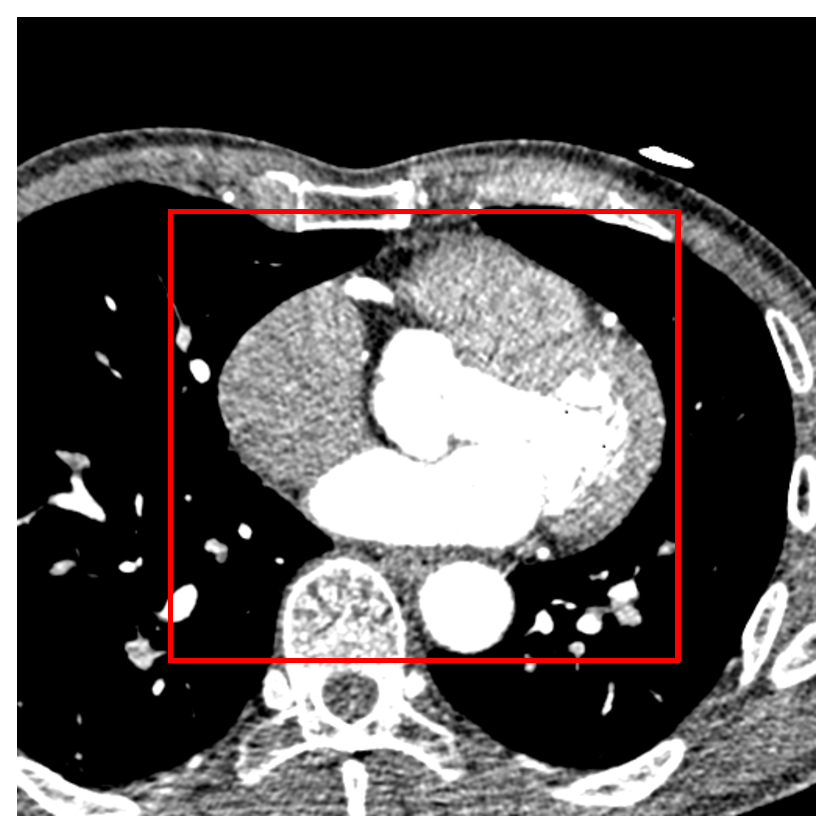
\includegraphics[width=1.5in]{../../Figures/coronary/ROI_Extraction}
% \caption[心脏区域的ROI提取]{心脏区域的ROI提取。}
% \label{fig:coronary_ROI}
\end{figure}
\end{frame}

\begin{frame}
\begin{itemize}
  \item \textbf{预处理结果}:
  \begin{enumerate}
    \onslide<1-2> \item 保护物体边缘的平滑处理($\text{传导参数} = 9.0$)
    \onslide<2> \item 阈值滤波($\text{TH}_{\text{lower}} = 160$, $\text{TH}_{\text{upper}} = 600$)
  \end{enumerate}
\end{itemize}
\begin{columns}[b,onlytextwidth]
\begin{column}{.5\textwidth}
\onslide<1-2> \begin{figure}
\centering
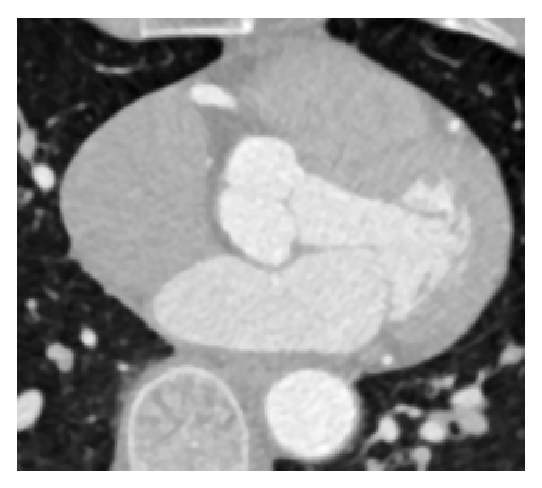
\includegraphics[height=1.5in]{../../Figures/coronary/smooth.eps}
\end{figure}
\end{column}
\begin{column}{.5\textwidth}
\onslide<2> \begin{figure}
\centering
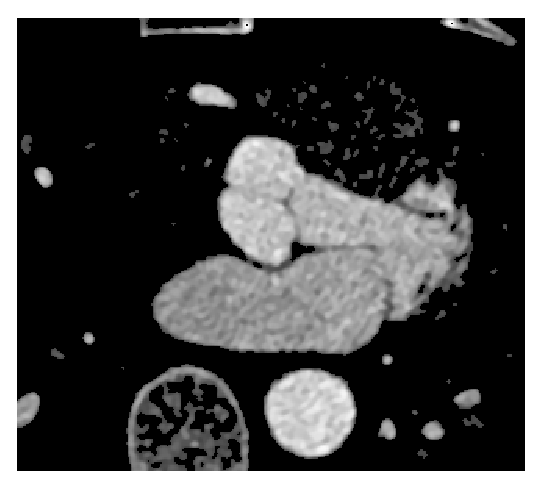
\includegraphics[height=1.5in]{../../Figures/coronary/threshold.eps}
\end{figure}
\end{column}
\end{columns}
\end{frame}

\begin{frame}
\begin{itemize}
  \item \textbf{特征图像计算}:
  \begin{enumerate}
    \onslide<1-2> \item 基于Gaussian核运算所得到的梯度图像($\sigma = 0.9$)
    \onslide<2> \item 通过S函数实现的像素亮度非线性映射($m = -80$, $n = 120$)
  \end{enumerate}
\end{itemize}
\begin{columns}[b,onlytextwidth]
\begin{column}{.5\textwidth}
\onslide<1-2> \begin{figure}
\centering
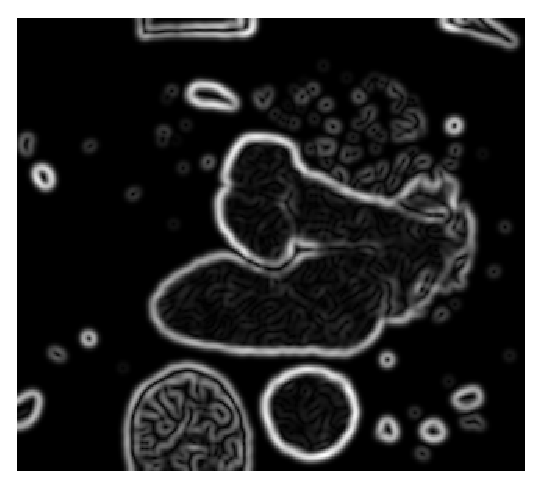
\includegraphics[height=1.5in]{../../Figures/coronary/gradient.eps}
\end{figure}
\end{column}
\begin{column}{.5\textwidth}
\onslide<2> \begin{figure}
\centering
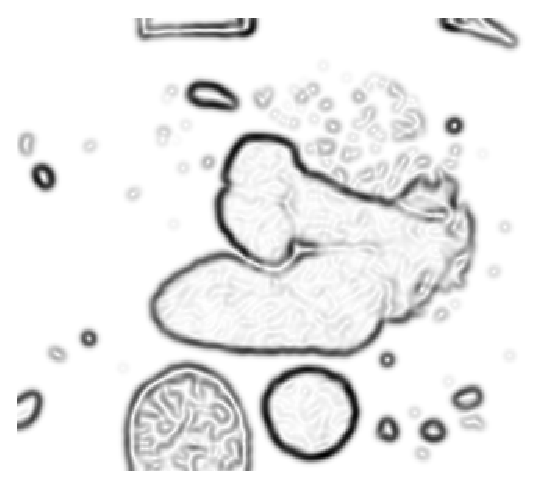
\includegraphics[height=1.5in]{../../Figures/coronary/sigmoid.eps}
\end{figure}
\end{column}
\end{columns}
\end{frame} 

\begin{frame}
\begin{itemize}
  \item \textbf{水平集演进过程}:
  \begin{enumerate}
    \onslide<1-3> \item 通过快速步进算法生成的初始水平集围线
    \onslide<2-3> \item 由CURVES驱动的围线演进结果(迭代次数:$50$)
    \onslide<3> \item 对演进结果进行二值阈值滤波处理后的结果
  \end{enumerate}
\end{itemize}
\begin{columns}[b,onlytextwidth]
\begin{column}{.3\textwidth}
\onslide<1-3> \begin{figure}
\centering
\setlength{\fboxrule}{0.1pt}
\setlength{\fboxsep}{0cm}
\fbox{
\includegraphics[width=1.2in]{../../Figures/coronary/fastmarching.eps}}
\end{figure}
\end{column}
\begin{column}{.3\textwidth}
\onslide<2-3> \begin{figure}
\centering
\setlength{\fboxrule}{0.1pt}
\setlength{\fboxsep}{0cm}
\fbox{
\includegraphics[width=1.2in]{../../Figures/coronary/curves.eps}}
\end{figure}
\end{column}
\begin{column}{.3\textwidth}
\onslide<3> \begin{figure}
\centering
\setlength{\fboxrule}{0.1pt}
\setlength{\fboxsep}{0cm}
\fbox{
\includegraphics[width=1.2in]{../../Figures/coronary/final.eps}}
\end{figure}
\end{column}
\end{columns}
\end{frame} 

\begin{frame}
\begin{itemize}
  \item \textbf{冠状动脉表面模型}:
\end{itemize}
\begin{figure}
\centering
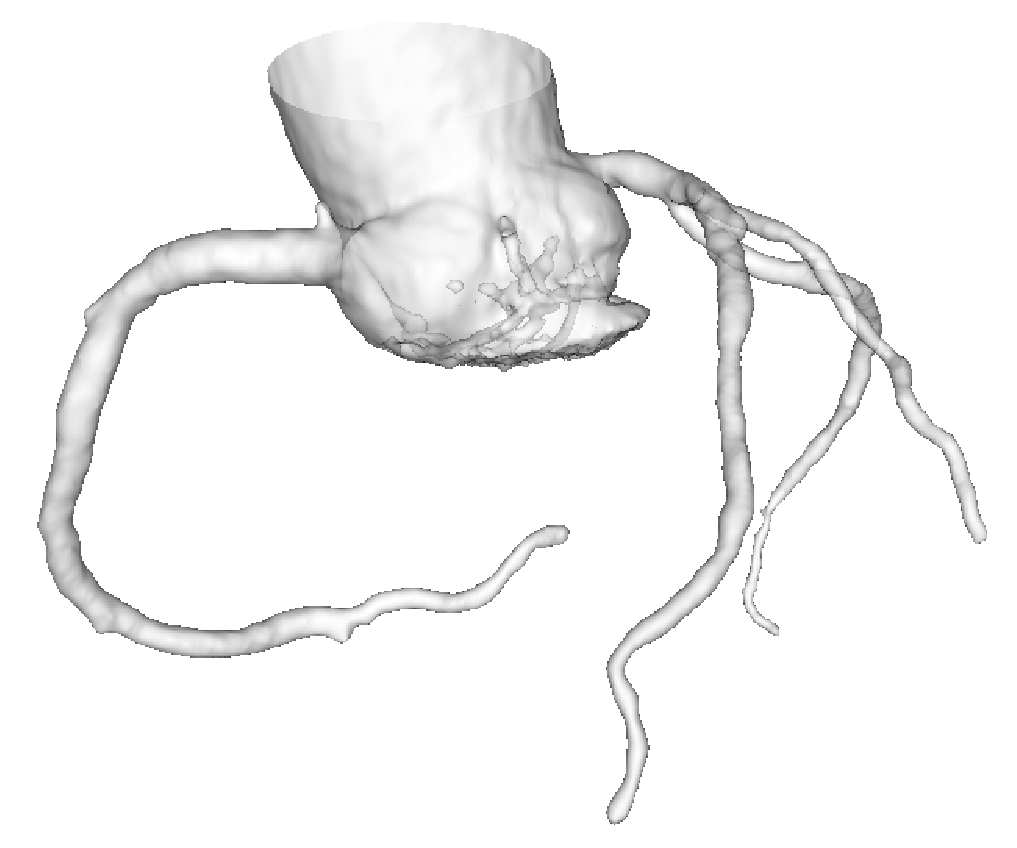
\includegraphics[width=1.5in]{../../Figures/coronary/model}
% \caption[心脏区域的ROI提取]{心脏区域的ROI提取。}
% \label{fig:coronary_ROI}
\end{figure}
\end{frame} 

% \begin{frame}

% \end{frame} 
